\documentclass[tikz,border=2pt]{standalone}
\usepackage{amsmath,amssymb}
\usepackage{tikz}
\usetikzlibrary{arrows.meta}

\begin{document}
% Two tosses of a coin picked at random (fair or biased): given which coin was chosen, the
% tosses are independent; unconditionally they are not, because the first toss hints at the coin.
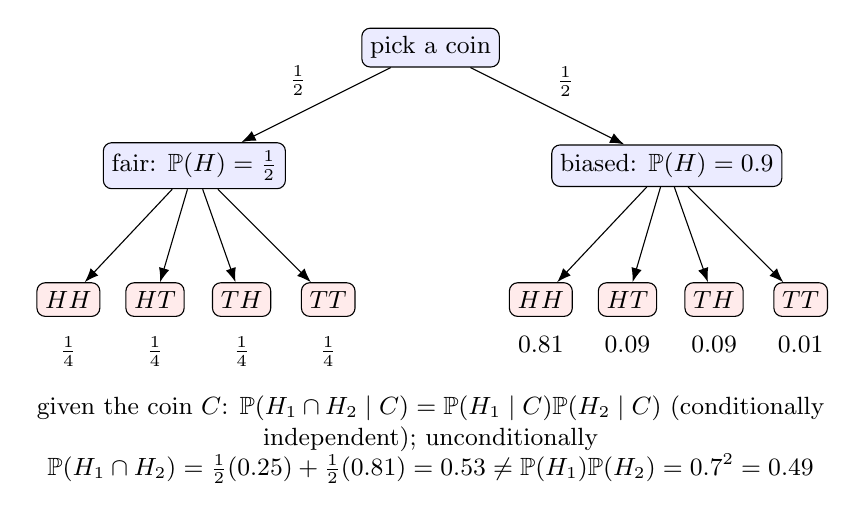
\begin{tikzpicture}[every node/.style={font=\small}, >={Latex[length=1.8mm]}, lvl/.style={draw, rounded corners=3pt, fill=blue!8, inner sep=3pt}]
	\node[lvl] (root) at (0,0) {pick a coin};
	\node[lvl] (F) at (-3,-1.5) {fair: $\mathbb{P}(H)=\tfrac12$};
	\node[lvl] (B) at (3,-1.5) {biased: $\mathbb{P}(H)=0.9$};
	\draw[->] (root) -- (F) node[midway, above left, font=\small] {$\tfrac12$};
	\draw[->] (root) -- (B) node[midway, above right, font=\small] {$\tfrac12$};
	\foreach \c/\x/\p/\q in {F/-3/0.5/0.5, B/3/0.9/0.1} {
		\node[lvl, fill=red!8] (\c HH) at (\x-1.6,-3.2) {$HH$};
		\node[lvl, fill=red!8] (\c HT) at (\x-0.5,-3.2) {$HT$};
		\node[lvl, fill=red!8] (\c TH) at (\x+0.6,-3.2) {$TH$};
		\node[lvl, fill=red!8] (\c TT) at (\x+1.7,-3.2) {$TT$};
		\draw[->] (\c) -- (\c HH);
		\draw[->] (\c) -- (\c HT);
		\draw[->] (\c) -- (\c TH);
		\draw[->] (\c) -- (\c TT);
	}
	\node[font=\small, anchor=north] at (-4.6,-3.55) {$\tfrac14$};
	\node[font=\small, anchor=north] at (-3.5,-3.55) {$\tfrac14$};
	\node[font=\small, anchor=north] at (-2.4,-3.55) {$\tfrac14$};
	\node[font=\small, anchor=north] at (-1.3,-3.55) {$\tfrac14$};
	\node[font=\small, anchor=north] at (1.4,-3.55) {$0.81$};
	\node[font=\small, anchor=north] at (2.5,-3.55) {$0.09$};
	\node[font=\small, anchor=north] at (3.6,-3.55) {$0.09$};
	\node[font=\small, anchor=north] at (4.7,-3.55) {$0.01$};
	\node[anchor=north, align=flush center, text width=10cm] at (0,-4.3) {given the coin $C$: $\mathbb{P}(H_1\cap H_2\mid C)=\mathbb{P}(H_1\mid C)\mathbb{P}(H_2\mid C)$ (conditionally independent); unconditionally $\mathbb{P}(H_1\cap H_2)=\tfrac12(0.25)+\tfrac12(0.81)=0.53\neq \mathbb{P}(H_1)\mathbb{P}(H_2)=0.7^2=0.49$};
\end{tikzpicture}
\end{document}
